% -*- coding: utf-8 -*-
\iffalse
\chapter{\Bezier 曲線}
図\ref{svg-bezier-interactive}は\Bezier 曲線の性質を確認するために制御点をド
ラッグして動かしたり、値を直接設定することができるようにしています。
\ShowGraphicPT{0.9}{ht}{bezier-interactive}
{\Bezier 曲線をインターラクティブに操作する}{svg-bezier-interactive}
このリストは次のようになっています。
\XMLListN{\Bezier 曲線をインターラクティブに操作する}
  {svg-bezier-interact-3-sjis}{bezier-interractive}
\begin{itemize}
 \item \LineR{globalsS}{fillInfoP2}は\Bezier 曲線の初期値や中を塗る色を
       指定や後で使うためのグローバル変数を定義しています。
\ListSub{globalsS}{fillInfoP2}
\begin{itemize}
 \item \LineR{controlPoints1}{controlPoints2}では
       \Bezier 曲線の制御点の位置とその点の色を指定しています。
 \item \LineR{fillInfoS}{fillInfoE}は「\Bezier 曲線が4つの制御点を含む最小
       の凸集合の中にある」という性質を確認すために(一般的には)四角形の
       内部の色と不透明度を定義しています。初めのもは全体の\Bezier 曲線
       のものを、後の二つは初めの\Bezier 曲線を途中の点で分割した\Bezier
       曲線のそれぞれの制御点からなる凸包を示すために使います。
 \item \Lines{fillInfoQ1}{fillInfoQ2}は制御点の初めの3点と後の3点から構
       成される2次の\Bezier 曲線を表示するパラメータを定義しています。
\end{itemize}
 \item \LineR{initS}{initE}は\SVG がロードした後、図形を初期化するための関数です。
\ListSub{initS}{initE}
\begin{itemize}
 \item \Line{canvas}では内部に含まれる\SVG のDOMでの位置を得ています。
       \Event{mousemove}のイベントはこのオブジェクトにだけ設定さ
       れます(\Line{addEventmousemove})。このオブジェクトの子ノードで発
       生したイベントをこの関数で処理することができます。
 \item このノードに対し\LineR{rectS}{rectE}で定義される長方形を子ノードと
       して付け加えます。

       \LineR{rectS}{rectE}では\Bezier 曲線を移動できる範囲の長方形を定
       義しています。
 \item \LineR{auxLineS}{auxLineE}では\Bezier 曲線の制御点から定義できる凸
       集合を示すオブジェクトを作成しています。色などの情報は
       \LineR{fillInfoS}{fillInfoE}で与えています。位置はこのあとのプロ
       グラムで計算して設定します。
 \item 右の部分にある位置を示すテキストボックスなどは
       \LineR{makeTR}{makeInput}で作成しています。
\begin{itemize}
 \item \Line{makeTR}で\TagH{tr}要素を作成し、点の名前を表示する
       \TagH{td}要素(制御点の色と文字の色を合わせるために
       制御点のデータが入っている配列(\texttt{IPos}を利用している)と
       \TagJ{textNode} を作成しています(\Line{makeText})。
 \item 点の位置を示す2つのテキストボックスはここで定義しているオブジェク
       ト\texttt{BoxP}で実現しています(\LineR{BoxPS}{BoxPE})。オブジェクトか
       ら新規のもの(インスタンス)を作成するためには\TagJ{new} をそのオブ
       ジェクトの前につけます。
\end{itemize}
 \item 制御点の図形もここで定義しているオブジェクト\texttt{Point}を用いて作成
       しています(\LineR{setControlPointsS}{setControlPointsE})。
 \item \LineR{setMidPointsS}{setMidPointsE}では制御点を順に結んで
       得られる点、また、それらの隣り合う点から得られる新しい点のオブジェ
       クトを作成しています。ここでは位置は設定していません。
 \item 制御点の中間の位置を決める値の\texttt{Portion}の値を\texttt{1/2}
       に設定します(\Line{setPortion})。
 \item 最後に、これらの位置から目的の図形を作成する関数
       \texttt{setControlPointsS}を呼び出して(\Line{refreshRegion})初期
       化が終了します。
\end{itemize}
 \item \LineR{PointsS}{PointsE}は制御点を示すオブジェ
       クトを定義している部分です。
\ListSub{PointsS}{readCxCyE}
\begin{itemize}
 \item \LineR{PointsS}{PointsE}はオブジェクトを作成する関数(コン
       ストラクタ)です。このコンストラクタはメンバーにSVG の円のオブジェ
       クトを持ちます。この親のオブジェクトと円の中心の位置、塗りつぶし
       の色、半径とそれにつけるイベントを引数に取ります。
 \item \LineR{makeCircleS}{makeCircleE}で円を作成し、\texttt{Circle}メン
       バに代入します。\TagJ{this}は現在作成しているオブジェクトを示す識
       別氏です。
 \item また、円の中心位置をメンバ\texttt{x}と\texttt{y}に代入します
       (\Lines{setCx}{setCy})。
 \item \JS のメソッドは
\begin{center}
 オブジェクト名\texttt{.}\TagJ{prototype}\texttt{.}
       関数名\texttt{= function(引数リスト)\{関数本体\}}
\end{center}
の形で宣言します。
 \item ここではメソッドとして\texttt{setPos}、\texttt{movePos}、
       \texttt{getPos}と\texttt{toSt}の4つが定義されています。
 \item メソッド\texttt{setPos}は与えられたテキストボックスの数値から制御
       点の位置を設定します。引数として与えられたテキストボックスのオブ
       ジェクトから値をそのオブジェクトの\texttt{Circle}の\Tag{circle}の
       中心位置を設定します(\Line{setCenter})。

       また、それらの値をプロパティの\texttt{x}と\texttt{y}に数値として格
       納します(\Lines{refreshX}{refreshY})。
 \item メソッド\texttt{movePos}は与えられた引数の位置に点を移動させます
       (\LineR{movePosS}{movePosE})。メソッド\texttt{setPos}とほとんど同
       じことをしています。
 \item メソッド\texttt{getPos}は点の位置を\texttt{Circle}に格納されてい
       る属性からそのオブジェクトのプロパティ\texttt{x}と\texttt{y}に設
       定するメソッドです(\LineR{getPosS}{getPosE})。ドラッグした後に使用します。
 \item メソッド\texttt{toSt}はプロパティの円の要素の中心位置を\texttt{,}
       でつないだ文字列に変換するものです(\LineR{toSt}{readCxCyE})。
\end{itemize}
 \item オブジェクト\texttt{BoxP}は制御点の座標を表示する
       テキストボックスの組を表すオブジェクトを定義します。
\ListSub{BoxPS}{BoxPValE}
\begin{itemize}
 \item プロパティ\texttt{x}と
       \texttt{y}にそれぞれテキストボックスを\TagH{td}内に作成し
       指定された要素内に設定します(\LineR{BoxPS}{BoxPE})。
 \item メソッド\texttt{setVal}はドラッグして移動された円の位置をテキスト
       ボックスに設定するためのものです(\LineR{BoxPValS}{BoxPValE})。
       指定された円の親のオブジェクトの\texttt{x}と\texttt{y}を設定した
       (\Line{setTextBoxValfromObj1})後、テキストボックスの値を変更します。 
\end{itemize}
 \item 次の部分は画面の更新をするための関数です。
\ListSub{setPosS}{RefreshRegionE}
\begin{itemize}
 \item \LineR{setPosS}{setPosE}の関数\texttt{SetPos()}は右にある「設定」
       ボタンが押されたときに呼び出される関数です。テキストボックスの値
       を制御点の中心に設定した(\Line{setpos})あと、画面の更新をする関
       数\texttt{RefreshRegionN()}を呼び出します。
 \item \LineR{RefreshRegionS}{RefreshRegionE}の関数
       \texttt{RefreshRegion}は制御点をドラッグしているときに呼び出され
       ます。制御点の画面の位置をテキストボックスに設定した
       (\Line{setTextBoxValfromObjs})あと、画面の更新をする関
       数\texttt{RefreshRegionN()}を呼び出します。
\end{itemize}
 \item 関数\texttt{RefreshRegionN()}は更新した制御点の位置から残りの点の
       位置を計算し、\Bezier 曲線の性質を確認するための凸な四角形を表示
       します。
\ListSub{RefreshRegionNS}{RefreshRegionNE}
\begin{itemize}
 \item \LineR{checkPS}{checkPE}では\texttt{Portion}の値が$0$と$1$の間に
       あるかどうかをチェックし、範囲外の場合には警告を出し、その値を\texttt{1/2}に
       設定します。
 \item \LineR{setInitialPathS}{setInitialPathE}では制御点の位置を求
       めています。

       それを元に現在の制御点による\Bezier 曲線を描きます
       (\Line{drawBeziere})。
 \item \LineR{calcMidPointsS}{calcMidPointsE}では制御点を元にそれらの
       中点の位置を計算し、中点を結んで得られる直線の\Tag{path}の属性値
       を作成しています。すべての直線を一つの\TagF{path}で描いています。
 \item \LineR{drawQBezierS}{drawQBezierE}では補助の2次の\Bezier 曲線を設
       定しています。
 \item 最後に、制御点から構成される最小の凸集合と細分された\Bezier 曲線
       を含む最小の凸集合を計算する関数\texttt{PaintRegion()}を呼び出し
       ています(\LineR{showConvexregion1}{showConvexregion3})。
\end{itemize}
 \item 関数\texttt{PaintRegion()}は与えられた4点からそれを含む最小の
       凸集合を決めます(\LineR{PaintRegionN}{PaintRegionE})。

       ここでは4点からなる集合なので個別にチェックすることにします。基本
       的な考え方は次の通りです。
\begin{itemize}
 \item 2点$\textrm{A}$と$\textrm{B}$を結ぶ直線は平面を二つの領域に分けま
       す。このうち、点$\textrm{A}$から$\textrm{B}$に向かうとき左側に見
       える方を正領域、他方を負領域と呼ぶことにします。
 \item 3直線$\textrm{P}_0\textrm{P}_1$、$\textrm{P}_1\textrm{P}_2$と
       $\textrm{P}_2\textrm{P}_0$を考えますと平面は7つの領域に分割されま
       す。図\ref{region-sign}は点$\textrm{P}_2$が直線
       $\textrm{P}_0\textrm{P}_1$の正領域にあるときに3本の直線による正領
       域、負領域がどうなるかを示したものです。3本の直線の正領域($+$)、
       負領域($-$)をこの順に表した記号で示しています。
\setlength{\unitlength}{0.5cm}
\begin{figure}[ht]\hspace*{\fill}
 \begin{picture}(16,15)(-4,-4)
  \put(-4,-4){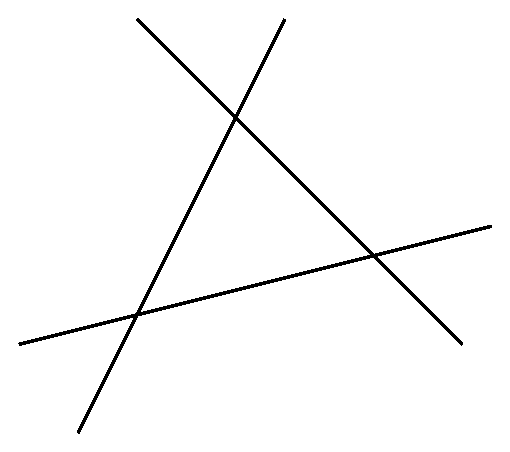
\includegraphics{Appendix/region.eps}}
  \put(0,-0.75){$\mathrm{P}_0$}
  \put(8,1.){$\mathrm{P}_1$}
  \put(3,8){$\mathrm{P}_2$}
  \put(3,3){$+++$}
  \put(4,-1){$-++$}
  \put(7,6){$+-+$}
  \put(2,10){$+--$}
  \put(10,1){$--+$}
  \put(-2,3){$++-$}
  \put(-4,-2.5){$-+-$}
 \end{picture}\hspace*{\fill}
\caption{3直線で区切られた領域の符号}\label{region-sign}
\end{figure}
 \item $\textrm{P}_3$がこれらのどの領域に入るかでこの4点を含む最小の凸集
       合の形が決まります。たとえば$++-$と示された領域では四角形
       $\textrm{P}_0\textrm{P}_1\textrm{P}_2\textrm{P}_3$が求めるもので
       すが$+--$と示された領域では$\textrm{P}_0\textrm{P}_1\textrm{P}_3$
       が求めるものになります。
 \item 直線$\textrm{AB}$に対し、点$\textrm{C}$がその正領域に属するかどうか
       は3角形$\textrm{ABC}$の符号を調べればわかります。その関数が
       \LineR{getSignS}{getSignE}で定義されている関数\texttt{getSign()}です。
 \item 図\ref{region-sign}を見ながら判定ができることを確認してください。
\end{itemize}
 \item 残りの\JS の部分はドラッグの処理をしています。
\ListSub{mousedownS}{mouseupE}
\begin{itemize}
 \item \LineR{mousedownS}{mousedownE}は\Event{mousedown}の処理をしています。
 \item \Line{moveTargetUp}ではイベントが発生したオブジェクトを一番上に表
       示するために\DOMM{appendChild}を用いています。
 \item イベントが発生した位置と発生したオブジェクトの中心の座標との差を
       保存しています(\Lines{savePosx}{savePosy})。これはドラッグ中に円
       の動きが不自然にならないようにするためです。
 \item 最後に\Line{addEventmousemove}でSVG の領域に\Event{mousemove}のイ
       ベント処理関数を割り当てています。
 \item \LineR{mousemoveS}{mousemoveE}でに\Event{mousemove}のイ
       ベント処理関数を定義しています。\Event{mousemove}のイベントで得ら
       れる位置には\Event{mousedown}で得られた補正値を加えていることに注
       意してください。
 \item その後、画面の書き直す関数\texttt{RefreshRegion()}を呼び出してい
       ます。
 \item \LineR{mouseupS}{mouseupE}では\Event{mouseup}の処理を定義していま
       す。ここでは\Event{mousemove}のイベント処理関数の割り当てを解除し
       ています。
\end{itemize}
\end{itemize}
%\ListSub{}{}

\fi
